\documentclass[a4paper, 11pt, openany]{report}


\usepackage{ensa-a} %%%%Important to use functionalities used in the vid. 



\begin{document}

\pagedegarde{ENSA4/GI/23-24}{d'année}{Abdelhak Mekaoui}{Adil Abbadi}{Génie Informatique}{Conception, Développement et Déploiement d'un Chatbot Inte lligent et d'une Plate forme E-Learning}{M. Prof 1}{M. Encadrent}{asset/sotemag.png}{0.1}{M. Prof 2}{M. Prof 3}{10/06/2024}

\newpage
\listoffigures
\listoftables
\listofcodes
\newpage

\tableofcontents
\newpage

\begin{remerciement}

\lettrine[nindent=0em, slope=-.5em]{\color{Eblue}F}{élicitations} à toute l'équipe de SOTEMAG pour votre dévouement et votre soutien constants. Nous sommes profondément reconnaissants pour l'opportunité de travailler avec vous et pour tout ce que nous avons appris grâce à votre expertise.

\vspace{0.5cm}

\lettrine[nindent=0em, slope=-.5em]{\color{Eblue}U}{nis} par notre engagement envers l'excellence, nous sommes reconnaissants d'avoir fait partie d'une équipe aussi dynamique et talentueuse que la vôtre. Votre passion pour l'innovation nous a inspirés à repousser nos limites et à atteindre de nouveaux sommets.

\vspace{0.5cm}

\lettrine[nindent=0em, slope=-.5em]{\color{Eblue}C}{ollaborer} avec vous a été une expérience enrichissante. Votre professionnalisme et votre soutien inestimable ont été des facteurs essentiels pour notre développement professionnel. Merci d'avoir été des mentors exceptionnels pour nous.

\vspace{0.5cm}

\lettrine[nindent=0em, slope=-.5em]{\color{Eblue}K}{udos} à toute l'équipe de SOTEMAG pour votre esprit d'équipe et votre détermination à surmonter les défis. Votre créativité et votre ingéniosité ont été une source d'inspiration constante pour nous tous.

\vspace{0.5cm}

\lettrine[nindent=0em, slope=-.5em]{\color{Eblue}U}{nifiés} tous, chaque jour était une aventure passionnante. Merci d'avoir créé un environnement de travail stimulant où nous avons pu grandir et nous épanouir professionnellement.

\end{remerciement}

\newpage %%%Warning!!!! Important before starting your report

\chapter{Introduction présentative :}
\section{Présentation de l'entreprise :}
Fondée en 1984 sous la forme d'une société anonyme, SOTEMAG (Société Technique de Matériel Agricole) a amorcé son parcours en se concentrant sur la fabrication et la distribution d'une gamme variée de composants mécaniques, en mettant particulièrement en avant la célèbre pompe DELTAX. Évoluant avec le temps, l'expertise de SOTEMAG s'est progressivement centrée sur la production de la pompe ALEXY, en parallèle avec l'élargissement de son portefeuille d'équipements agricoles.

Stratégiquement implantée au cœur de la zone industrielle dynamique d'Ait Melloul, à seulement 15 kilomètres de la vibrante ville d'Agadir, l'usine de fabrication de SOTEMAG s'épanouit au sein d'un véritable havre agricole. Ce choix géographique a été influencé par le statut agricole prédominant de la région, faisant d'Ait Melloul un emplacement idéal. Avec une base de consommateurs largement composée d'agriculteurs locaux, ce lieu garantit un accès direct à une clientèle diversifiée.

Dotée d'une usine entièrement équipée, les capacités de production de SOTEMAG englobent une variété d'ateliers, allant de la fonderie à la fabrication numérique et à la tuyauterie. Cette infrastructure intégrée constitue un avantage distinctif, permettant à l'entreprise de livrer des produits d'une qualité inégalée qui transcendent les frontières régionales. En répondant aux demandes des marchés marocains et en satisfaisant constamment les besoins des clients, SOTEMAG a acquis une réputation qui dépasse largement son environnement immédiat.

\begin{table}
\centering
\renewcommand*{\arraystretch}{1.5}
\begin{tabular}{|>{\columncolor{Eblue!10}}c|p{8cm}|}
\hline
Dénomination sociale & Société technique de matériel agricole\\
\hline
Statut juridique & Société Anonyme \\
\hline
Siège sociale & Km 2,5 Route de Biougra BP 114 BP 86150 Ait-Melloul\\
\hline
Secteur d'activité & Les équipements agricoles \\
\hline
Capital & 40 000 000 DHS\\
\hline
PDG & Moulay Mohamed Elmessaoudi\\
\hline
Effectif & 300\\
\hline
Adresse email & \href{mailto:sotemag@menara.ma}{\ttfamily sotemag@menara.ma}\\
\hline
Site web & \href{https://sotemag.com}{\ttfamily sotemag.com}\\
\hline
Téléphone & \href{tel:+212528240134}{\ttfamily +212528240134/70} | \href{tel:+212528240244}{\ttfamily +212528240244/45} \\
\hline
\end{tabular}
\caption{Fiche signalétique}
\end{table}

\section{Domaine d'activités :}

\subsection{Fabrication des pompes à axe vertical :}
Fort d'une expérience de plus de 35 ans, SOTEMAG a su mettre à profit son savoir-faire pour concevoir et exporter ses propres gammes de pompes ALEXY et DELTAX. Dans le but de parfaire son offre dans le domaine du pompage, SOTEMAG propose désormais des groupes électropompes d'une qualité supérieure. Ces groupes électropompes sont issus des marques renommées EBARA et ROVATA, gages de fiabilité et de performance.

\subsection{Matériel Agricole :}
SOTEMAG propose un matériel agricole en parfaite conformité avec les normes internationales, tout en s'adaptant aux spécificités nationales. Grâce à sa réputation solide, SOTEMAG a établi des partenariats qualifiés et acquis une reconnaissance mondiale dans la fabrication d'équipements de haute qualité.

\subsection{Matériel de traitement et de nettoyage :}
SOTEMAG propose à sa clientèle une vaste gamme diversifiée d'équipements de traitement et de nettoyage reconnus à l'échelle mondiale, qui se distinguent par leurs performances et leur efficacité inégalées.

\subsection{Matérial de travaux publiques :}
SOTEMAG met à la disposition de sa clientèle une gamme étendue et diversifiée d'équipements de traitement et de nettoyage mondialement reconnus, distingués par leur performance exceptionnelle et leur efficacité remarquable.

\subsection{Tube en acier :}
SOTEMAG se distingue par son engagement à fournir des tubes d'une qualité exceptionnelle. Le processus de fabrication, bien que minutieux et élaboré, est le garant d'un résultat final des plus satisfaisants. Chaque étape est entreprise avec soin, depuis la sélection rigoureuse des matériaux jusqu'à l'application de techniques de fabrication de pointe. Ainsi, les tubes offerts par SOTEMAG incarnent la fusion parfaite entre la durabilité et les performances optimales, témoignant de l'effort continu de l'entreprise pour offrir le meilleur à ses clients.

\subsection{Service après-vente :}
Afin d'assurer une satisfaction optimale de la clientèle, SOTEMAG a instauré une structure de services après-vente hautement performante, composée de plus de 15 équipes autonomes, chacune équipée de matériel roulant. Cette mise en place garantit une réactivité remarquable à l'échelle du royaume, permettant à SOTEMAG de répondre de manière efficiente aux besoins de ses clients, où qu'ils se trouvent.

\section{L'usine SOTEMAG :}
SOTEMAG abrite une usine idéalement située le long de la route de Taroudant. Cet établissement de production est spécialement dédié à la fabrication de divers équipements de tournage, avec une attention particulière portée à la pompe à axe vertical ALEXY, une marque largement reconnue sur les marchés marocains.

Cette usine, en tant qu'unité de production complète et autonome, se distingue par un processus de fabrication minutieusement orchestré, qui relie ses composantes essentielles : l'unité de fonderie, l'unité d'usinage, l'unité de soudage, l'unité des machines CNC, et l'unité de montage et peinture. Ces entités indépendantes, disposant de ressources matérielles et humaines complètes, se révèlent être un atout cohérent et productif.

\begin{figure}[H]
\centering
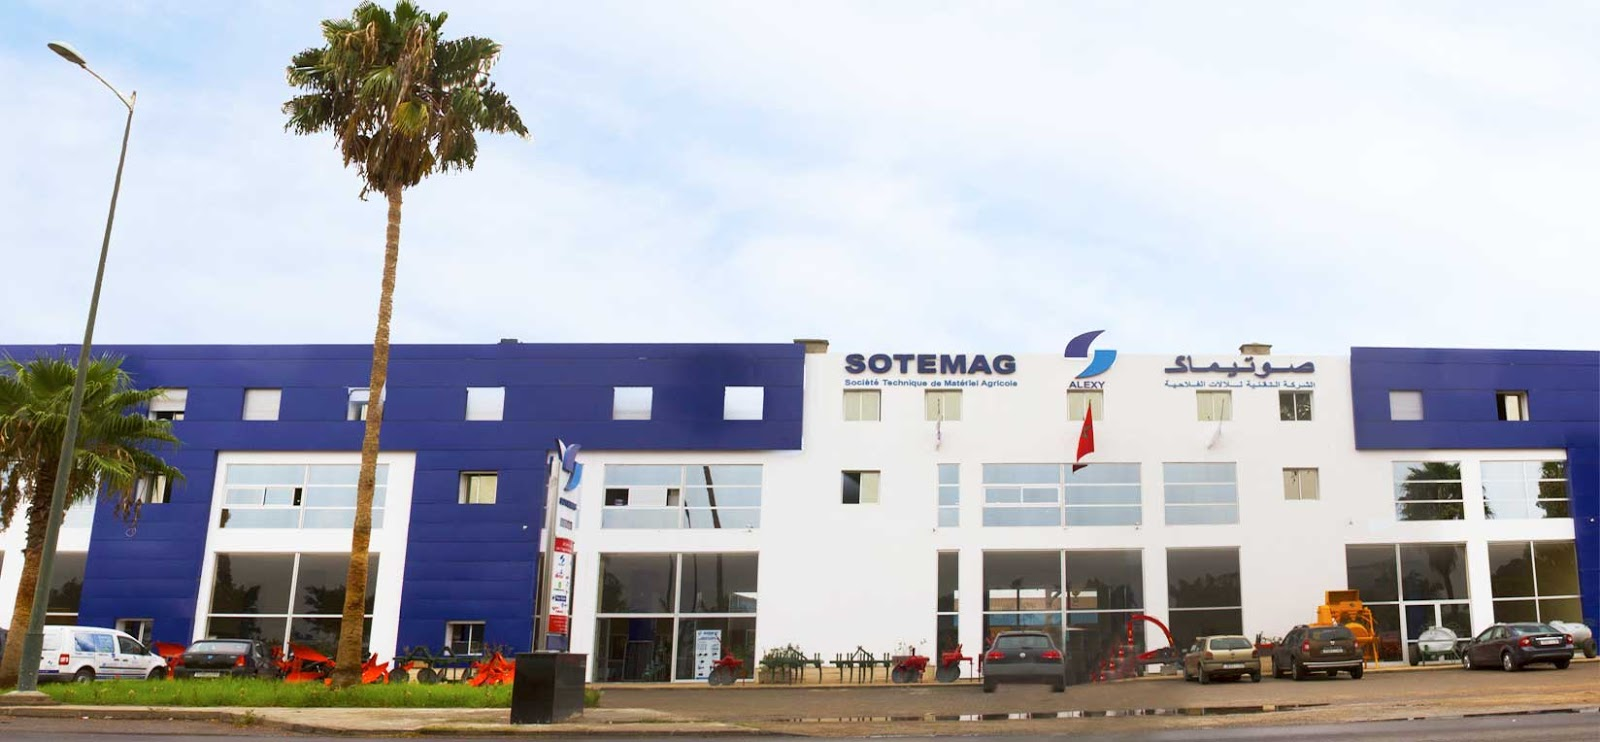
\includegraphics[scale=0.15]{asset/LocalSotemag.png}
\caption{Local de l'usine sotemag :}    
\end{figure}

Cette mise en synergie entre ces différentes unités favorise une production efficace et de haute qualité, tout en renforçant la capacité de SOTEMAG à offrir des produits répondant aux normes les plus exigeantes.
\setcounter{chapter}{2}
\chapter{Un titre très très très long, et exemple des codes dans ce thème :}

\begin{Code}
\begin{lstlisting}[language=python]
def Dreamers(k):
    for F in range(k):
        print("Dreamers")

def DreamersMatrix(k):
    Dmatrix = [["Dreamers" for _ in range(k)] for _ in range(k)]
    return Dmatrix

def HardWork(Dream, value):
    return Dream + value
\end{lstlisting}

\end{Code}

\end{document}
